\def\mytitle{MATRICES USING PYTHON}
\def\myauthor{R.Ramesh}
\def\contact{rameshrandhiglra@gmail.com}
\def\mymodule{Future Wireless Communication (FWC)}
\documentclass[10pt, a4paper]{article}
\usepackage[a4paper,outer=1.5cm,inner=1.5cm,top=1.75cm,bottom=1.5cm]{geometry}
\twocolumn
\usepackage{graphicx}
\graphicspath{{./images/}}
\usepackage[colorlinks,linkcolor={black},citecolor={blue!80!black},urlcolor={blue!80!black}]{hyperref}
\usepackage[parfill]{parskip}
\usepackage{lmodern}
\usepackage{tikz}
	\usepackage{physics}
%\documentclass[tikz, border=2mm]{standalone}
\usepackage{karnaugh-map}
%\documentclass{article}
\providecommand{\sbrak}[1]{\ensuremath{{}\left.#1\right]}}
\usepackage{tabularx}
\usepackage{circuitikz}
\usetikzlibrary{calc}
\usepackage{amssymb,amsfonts,amsthm,amsmath}
\usepackage{amssymb}
\renewcommand*\familydefault{\sfdefault}
\usepackage{watermark}
\usepackage{lipsum}
\usepackage{xcolor}
\usepackage{listings}
\usepackage{float}
\usepackage{titlesec}
\providecommand{\mtx}[1]{\mathbf{#1}}
\titlespacing{\subsection}{1pt}{\parskip}{3pt}
\titlespacing{\subsubsection}{0pt}{\parskip}{-\parskip}
\titlespacing{\paragraph}{0pt}{\parskip}{\parskip}
\newcommand{\figuremacro}[5]{
    \begin{figure}[#1]
        \centering
        \includegraphics[width=#5\columnwidth]{#2}
        \caption[#3]{\textbf{#3}#4}
        \label{fig:#2}
    \end{figure}
}
\providecommand{\norm}[1]{\left\lVert#1\right\rVert}
\newcommand{\myvec}[1]{\ensuremath{\begin{pmatrix}#1\end{pmatrix}}}
\let\vec\mathbf

\newcommand{\mydet}[1]{\ensuremath{\begin{vmatrix}#1\end{vmatrix}}}
\lstset{
frame=single, 
breaklines=true,
columns=fullflexible
}
%\thiswatermark{\centering \put(0,-90.0){\includegraphics[scale=0.5]{iit h.png}} }
\title{\mytitle}
\author{\myauthor\hspace{1em}\\\contact\\FWC22076\hspace{6.5em}IITH\hspace{0.5em}\mymodule\hspace{6em}September}
\date{}


\begin{document}
\maketitle
\paragraph{\textit{\large Problem statement: }\\The focus of an ellipse is at origin .The directrix is the line x=4 and eccentricity is 1/2. Then the length of the semi major axis is. \\}
 \section*{Construction}
 	\begin{center}
  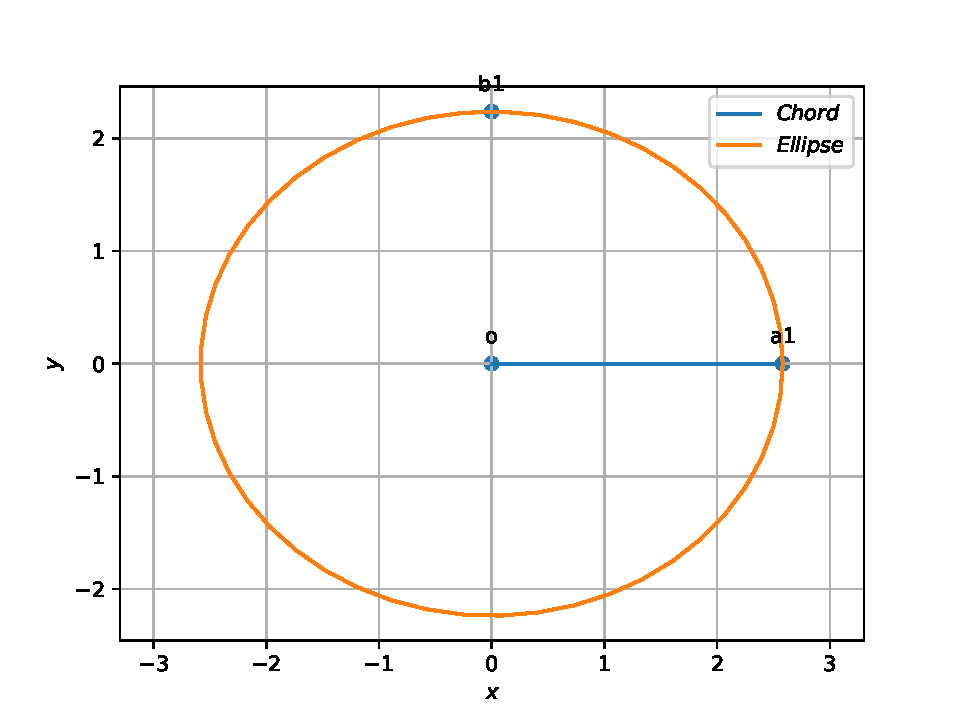
\includegraphics[scale=0.49]{figs16.pdf}
  
  Figure of construction
  	\end{center}
The input parameters for this construction are 
\begin{center}
\begin{tabular}{|c|c|c|}
	\hline
	\textbf{Symbol}&\textbf{Value}&\textbf{Description}\\
	\hline
	$\vec{F}$&\myvec{0\\0}&focus point\\[8pt]
	\hline
		${d}$&x=4&line of directrix\\[8pt]
	\hline
		$e$&{1/2}&value of eccntricity\\[8pt]
	\hline

\end{tabular}
\end{center}
\section*{Solution}
\textbf{Statement:}
The equation of  a conic with directrix $\vec{n}^{\top}\vec{x} = c$, eccentricity $e$ and focus $\vec{F}$ is given by 
\begin{align}
    \label{eq:conic_quad_form}
    \vec{x}^{\top}\vec{V}\vec{x}+2\vec{u}^{\top}\vec{x}+f=0
    \end{align}
where     
\begin{align}
  \label{eq:conic_quad_form_v}
\vec{V} &=\norm{\vec{n}}^2\vec{I}-e^2\vec{n}\vec{n}^{\top}, 
\\
\label{eq:conic_quad_form_u}
\vec{u} &= ce^2\vec{n}-\norm{\vec{n}}^2\vec{F}, 
\\
\label{eq:conic_quad_form_f}
f &= \norm{\vec{n}}^2\norm{\vec{F}}^2-c^2e^2
%\\
    \end{align}
  \begin{align}
		        \vec{n} = \myvec{1 \\ 0}, c = 4,
		  \end{align}      
		        \\
		     \begin{align}
		         \vec{F} = \myvec{0 \\ 0}
		     \end{align}    
		   
\textbf{} By substituting the values in above ,we get
\begin{align}
			 \vec{V}  = \myvec{\frac{3}{4}& 0
			    \\
			    0 & 1 }  
		    \end{align}
\\
\begin{align}
  \vec{u} = \myvec{1\\0}
\end{align}
\begin{align}
     f =-4
\end{align}
 \textbf{} since diagnoal elements of \textbf{V} are eigen values
\\
  \begin{align}
			    \lambda_2 = \norm{\vec{n}}^2= 1
		    \end{align}
		    \\
		     \begin{align}
			    \lambda_1 = \textbf{}(1-e^2)\lambda_2=\frac{3}{4}
		    \end{align}
		    \\
		   
\textbf{} Now, 
\begin{align}
		      f_0 &=\vec{u}^{\top}\vec{V}^{-1}\vec{u} -f \ne 0
		 \end{align}
   	    \begin{align}
		a = \sqrt{\frac{|f_0|}{|\lambda_1|}}
		    \end{align}
		     \begin{align}
		b = \sqrt{\frac{|f_0|}{|\lambda_2|}}
		    \end{align}
		 
\textbf{} By substituting the values in above ,we get
\begin{align}
       f_0=5
        \\
		a =2.58
		\\
		b=2.23
\end{align}
\textbf{} so, the length of semi major axis is $2.58$	
\end{document}